\documentclass[10pt]{article}\usepackage[]{graphicx}\usepackage[]{color}
%% maxwidth is the original width if it is less than linewidth
%% otherwise use linewidth (to make sure the graphics do not exceed the margin)
\makeatletter
\def\maxwidth{ %
  \ifdim\Gin@nat@width>\linewidth
    \linewidth
  \else
    \Gin@nat@width
  \fi
}
\makeatother

\definecolor{fgcolor}{rgb}{0.345, 0.345, 0.345}
\newcommand{\hlnum}[1]{\textcolor[rgb]{0.686,0.059,0.569}{#1}}%
\newcommand{\hlstr}[1]{\textcolor[rgb]{0.192,0.494,0.8}{#1}}%
\newcommand{\hlcom}[1]{\textcolor[rgb]{0.678,0.584,0.686}{\textit{#1}}}%
\newcommand{\hlopt}[1]{\textcolor[rgb]{0,0,0}{#1}}%
\newcommand{\hlstd}[1]{\textcolor[rgb]{0.345,0.345,0.345}{#1}}%
\newcommand{\hlkwa}[1]{\textcolor[rgb]{0.161,0.373,0.58}{\textbf{#1}}}%
\newcommand{\hlkwb}[1]{\textcolor[rgb]{0.69,0.353,0.396}{#1}}%
\newcommand{\hlkwc}[1]{\textcolor[rgb]{0.333,0.667,0.333}{#1}}%
\newcommand{\hlkwd}[1]{\textcolor[rgb]{0.737,0.353,0.396}{\textbf{#1}}}%
\let\hlipl\hlkwb

\usepackage{framed}
\makeatletter
\newenvironment{kframe}{%
 \def\at@end@of@kframe{}%
 \ifinner\ifhmode%
  \def\at@end@of@kframe{\end{minipage}}%
  \begin{minipage}{\columnwidth}%
 \fi\fi%
 \def\FrameCommand##1{\hskip\@totalleftmargin \hskip-\fboxsep
 \colorbox{shadecolor}{##1}\hskip-\fboxsep
     % There is no \\@totalrightmargin, so:
     \hskip-\linewidth \hskip-\@totalleftmargin \hskip\columnwidth}%
 \MakeFramed {\advance\hsize-\width
   \@totalleftmargin\z@ \linewidth\hsize
   \@setminipage}}%
 {\par\unskip\endMakeFramed%
 \at@end@of@kframe}
\makeatother

\definecolor{shadecolor}{rgb}{.97, .97, .97}
\definecolor{messagecolor}{rgb}{0, 0, 0}
\definecolor{warningcolor}{rgb}{1, 0, 1}
\definecolor{errorcolor}{rgb}{1, 0, 0}
\newenvironment{knitrout}{}{} % an empty environment to be redefined in TeX

\usepackage{alltt}

\usepackage{amsmath,amssymb,amsthm}
\usepackage{fancyhdr,url,hyperref}
\usepackage{graphicx}

\oddsidemargin 0in  %0.5in
\topmargin     0in
\leftmargin    0in
\rightmargin   0in
\textheight    9in
\textwidth     6in %6in
%\headheight    0in
%\headsep       0in
%\footskip      0.5in


\pagestyle{fancy}

\lhead{\textsc{Prof. McNamara}}
\chead{\textsc{SDS/MTH 220: Lecture Notes}}
\rhead{\textsc{September 27, 2017}}
\lfoot{}
\cfoot{}
%\cfoot{\thepage}
\rfoot{}
\renewcommand{\headrulewidth}{0.2pt}
\renewcommand{\footrulewidth}{0.0pt}

\newcommand{\ans}{\vspace{1in}}
\IfFileExists{upquote.sty}{\usepackage{upquote}}{}
\begin{document}
%\maketitle

\paragraph{Agenda}
\begin{enumerate}
  \itemsep0em 
  \item Finish notes from Monday
  \item Multiple regression
\end{enumerate}


\paragraph{Multiple Regression}

Multiple regression is a natural extension of simple linear regression.
\begin{itemize}
  \itemsep0in
  \item SLR: one response variable, one explanatory variable
  $$
    Y = \beta_0 + \beta_1 \cdot X + \epsilon, \text{ where } \epsilon \sim N(0, \sigma_\epsilon)
  $$
  \item MLR: one response variable, \emph{more than one} explanatory variable
  $$
    Y = \beta_0 + \beta_1 \cdot X_1 + \beta_2 \cdot X_2 + \cdots + \beta_p \cdot X_p + \epsilon, \text{ where } \epsilon \sim N(0, \sigma_\epsilon)
  $$
  \item Estimated coefficients (e.g. $\hat{\beta}_i$'s) now are interpreted in relation to (or ``conditional on'') the other variables
  \item $\beta_i$ reflects the \emph{predicted} change in $Y$ associated with a one unit increase in $X_i$, conditional upon the rest of the $X_i$'s.
  \item $R^2$ has the same interpretation (proportion of variability explained by the model)
\end{itemize}


\paragraph{Multiple Regression with a Categorical Variable}

Consider the case where $X_1$ is quantitative, but $X_2$ is an \emph{indicator} variable that can only be 0 or 1 (e.g. $coffeeTemp$). Then,
$$
  \hat{Y} = \hat{\beta}_0 + \hat{\beta}_1 \cdot X_1 + \hat{\beta}_2 \cdot X_2
$$
So then,
  \begin{align*}
    \text{For hot coffee, } \qquad \hat{Y} |_{ X_1, X_2 = 0} &= \hat{\beta}_0 + \hat{\beta}_1 \cdot X_1 \\
    \text{For cold coffee, } \qquad \hat{Y} |_{ X_1, X_2 = 1} &= \hat{\beta}_0 + \hat{\beta}_1 \cdot X_1 + \hat{\beta}_2 \cdot 1 \\
      &= \left( \hat{\beta}_0 + \hat{\beta}_2 \right) + \hat{\beta}_1 \cdot X_1
  \end{align*}
This is called a \emph{parallel slopes} model. [Why?]

\clearpage
\paragraph{Example: Class data}

Let's think back to the data we collected at the beginning of class again. We're going to try to predict how far from Smith you each were. We could start with a simple linear regression model,



\begin{knitrout}\footnotesize
\definecolor{shadecolor}{rgb}{0.969, 0.969, 0.969}\color{fgcolor}\begin{kframe}
\begin{alltt}
\hlstd{m1} \hlkwb{<-} \hlkwd{lm}\hlstd{(Distance_break}\hlopt{~}\hlstd{Num_languages,} \hlkwc{data}\hlstd{=us)}
\hlkwd{coef}\hlstd{(m1)}
\end{alltt}
\begin{verbatim}
##   (Intercept) Num_languages 
##     1404.6036      678.2473
\end{verbatim}
\begin{alltt}
\hlkwd{plotModel}\hlstd{(m1)}
\end{alltt}
\end{kframe}
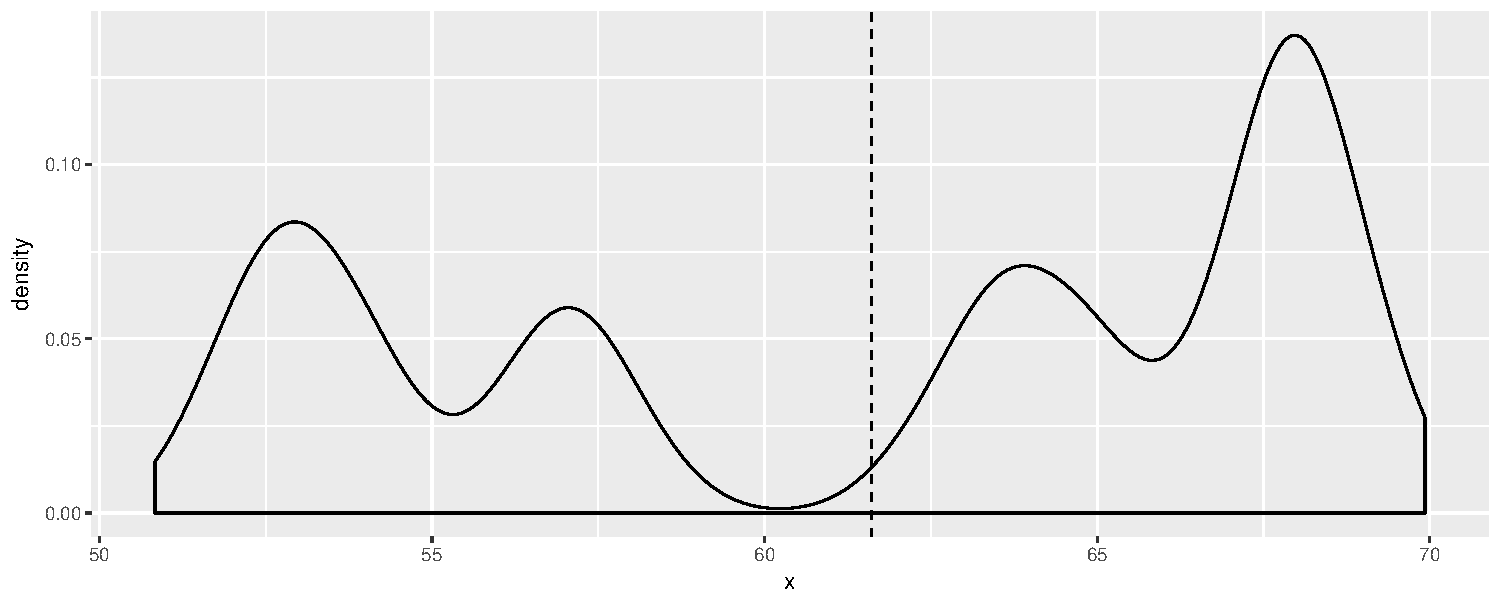
\includegraphics[width=\maxwidth]{figure/unnamed-chunk-2-1} 

\end{knitrout}

\begin{enumerate}
\itemsep1.2in
\item Write out the equation of the line
\item Interpret the slope and intercept of the line
\end{enumerate}

\clearpage
But, maybe we want to include some additional information. We can add variables into our linear model:

\begin{knitrout}\footnotesize
\definecolor{shadecolor}{rgb}{0.969, 0.969, 0.969}\color{fgcolor}\begin{kframe}
\begin{alltt}
\hlstd{m2} \hlkwb{<-} \hlkwd{lm}\hlstd{(Distance_break}\hlopt{~}\hlstd{Num_languages}\hlopt{+}\hlstd{Sheet_color,} \hlkwc{data}\hlstd{=us)}
\hlkwd{summary}\hlstd{(m2)}
\end{alltt}
\begin{verbatim}
## 
## Call:
## lm(formula = Distance_break ~ Num_languages + Sheet_color, data = us)
## 
## Residuals:
##     Min      1Q  Median      3Q     Max 
## -2885.6 -1464.4  -767.5   812.0  5643.1 
## 
## Coefficients:
##                   Estimate Std. Error t value Pr(>|t|)
## (Intercept)        1415.17    1201.08   1.178    0.247
## Num_languages       744.70     555.15   1.341    0.189
## Sheet_colorgreen    -34.75     974.41  -0.036    0.972
## Sheet_colorpurple  -383.68     925.93  -0.414    0.681
## 
## Residual standard error: 2352 on 34 degrees of freedom
##   (2 observations deleted due to missingness)
## Multiple R-squared:  0.05534,	Adjusted R-squared:  -0.02801 
## F-statistic: 0.664 on 3 and 34 DF,  p-value: 0.58
\end{verbatim}
\begin{alltt}
\hlkwd{plotModel}\hlstd{(m2)}
\end{alltt}
\end{kframe}
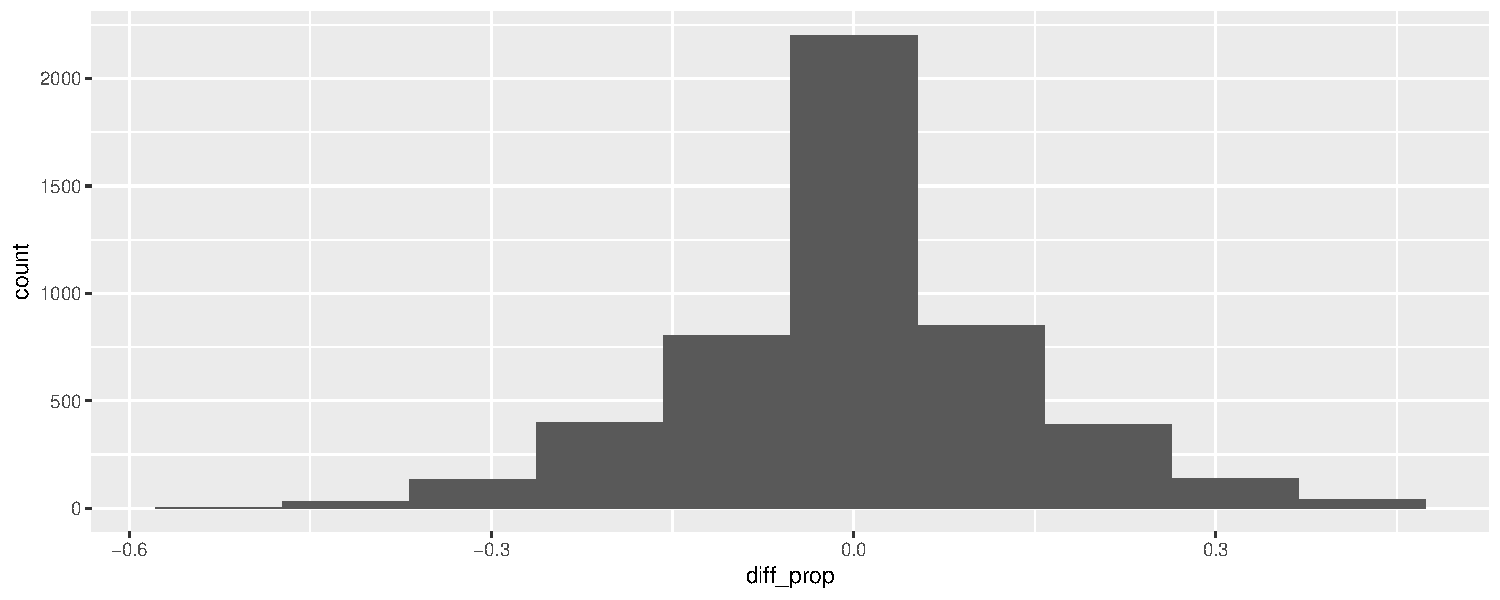
\includegraphics[width=\maxwidth]{figure/unnamed-chunk-3-1} 

\end{knitrout}
\clearpage
\begin{enumerate}
\itemsep1.2in
\item Write out the equation of the line
\item Interpret all the coefficeints in the model
\item Find the predicted value for yourself
\item Find your residual-- is it negative or positive?
 \vspace{1in}
\end{enumerate}

% \paragraph{Italian restaurant data}
% The Zagat guide contains restaurant ratings and reviews for many major world cities. We want to understand variation in the average $Price$ of a dinner in Italian restaurants in New York City. Specifically, we want to know how customer ratings (measured on a scale of 0 to 30) of the $Food$, $Decor$, and $Service$, as well as whether the restaurant is located to the $East$ or west of 5th Avenue, are associated with the average $Price$ of a meal. The data contains ratings and prices for 168 Italian restaurants in 2001.
% 
% <<message=FALSE,fig.show='hold', fig.height=4, size='footnotesize'>>=
% NYC <- read.csv("http://www.math.smith.edu/~bbaumer/mth241/nyc.csv")
% ggplot(data = NYC, aes(x = jitter(Service), y = Price)) +
%   geom_point(alpha = 0.5, size = 2) + geom_smooth(method = "lm", se = 0) +
%   xlab("Jittered service rating") + ylab("Average Price (US$)")
% lm(Price ~ Service, data = NYC)
% @
% 
% 
% \begin{enumerate}
%   \itemsep1.2in
%   \item Use {\tt qplot()} to examine the bivariate relationships between $Price$, $Food$ and $Service$.
%   \item What do you observe? Describe the form, direction, and strength of the relationships.
%   \item Use {\tt lm()} to build a SLR model for $Price$ as a function of $Food$. Interpret the coefficients of this model. How is the quality of the food at these restaurants associated with its price?
%   \item Build a parallel slopes model by conditioning on the $East$ variable. Interpret the coefficients of this model. What is the value of being on the East Side of Fifth Avenue?
%   \vspace{1in}
% \end{enumerate}
% 
% 
% 
% 
% <<echo=FALSE, size='footnotesize'>>=
% opts_chunk$set(tidy=TRUE, size='footnotesize')
% @
% 
% Let's build a model now for the $Price$ as a function of the $Food$ rating and the location relative to 5th Avenue. 
% 
% <<message=FALSE,fig.height=5, fig.show='hide'>>=
% require(mosaic)
% NYC <- read.csv("http://www.math.smith.edu/~bbaumer/mth241/nyc.csv")
% qplot(data = NYC, x = jitter(Food), y = Price) +
%   geom_smooth(method = "lm", se = 0)
% mod.fe <- lm(Price ~ Food + East, data = NYC)
% mod.fe
% @
% 
% 
% \begin{enumerate}
%   \itemsep0.7in
%   \item Interpret the coefficients of this model. What is the value of being on the East Side of Fifth Avenue?
%   \item Calculate the expected $Price$ of a restaurant in the East Village with a $Food$ rating of 23. 
%   \item Use \texttt{plotModel()} to visualize your model in the data space. 
%   
%   <<eval=FALSE>>=
% plotModel(mod.fe, xlab = "Jittered food rating", ylab = "Average Price (US$)", system = "ggplot2")
% @
%   
% \end{enumerate}


% \paragraph{Multiple Regression with a Second Quantitative Variable}
% If $X_2$ is a quantitative variable, then we have
% 
%   $$
%     \hat{Y} = \hat{\beta}_0 + \hat{\beta}_1 \cdot X_1 + \hat{\beta}_2 \cdot X_2
%   $$
% Notice that our model is no longer a line, rather it is a \emph{plane} that lives in three dimensions!
% 
% \paragraph{Italian Restaurants (continued)}
% 
% Now suppose that we want to improve our model by considering not only the quality of the $Food$, but also the quality of the $Service$. We can do this in {\tt R} by simply adding another variable to our regression model.
% 
% <<message=FALSE,fig.height=3, eval=TRUE>>=
% mod.fs <- lm(Price ~ Food + Service, data = NYC)
% coef(mod.fs)
% @
% 
% <<tidy=TRUE, eval=FALSE>>=
% fit.price <- makeFun(mod.fs)
% plotFun(fit.price(f,s) ~ f & s, surface=TRUE, f.lim=c(0,30), s.lim=c(0,30), alpha=0.5)
% @
% 
% <<tidy=TRUE, eval=FALSE>>=
% require(rgl)
% opacity <- 0.4
% with(NYC, plot3d(x = Food, y = Service, z = Price, type = "s", size = 0.3,
%     col = "blue", xlab = "Food Rating", ylab = "Service Rating",
%     zlab = "Price ($)"))
% coefs <- coef(mod.fs)
% planes3d(coefs["Food"], coefs["Service"], -1, coefs["(Intercept)"], alpha = opacity,
% col = "lightgray")
% @
% 
% \begin{enumerate}
%   \itemsep0.7in
%   \item Interpret the coefficients of this model. What does the coefficient of $Food$ mean in the real-world context of the problem? $Service$?
%   \item How important is $Service$ relative to $Food$? Is it fair to compare the two coefficients?
%   \item Use {\tt makeFun()} to find the expected $Price$ of a restaurant with a $Food$ rating of 21 but a $Service$ rating of 28. 
%   \item Calculate the residual for \href{http://www.zagat.com/r/san-pietro-new-york}{San Pietro}. Is it overpriced? 
%   <<>>=
% filter(NYC, Restaurant == "San Pietro")
% @
% 
% 
%   \item What if we added all three explanatory variables to the model? What geometric shape would we have then? 
% 
% 
% <<tidy=TRUE, eval=FALSE>>=
% with(NYC, plot3d(x = Food, y = Service, z = Price, type = "s", size = 0.8,
%     col = "blue", xlab = "Food Rating", ylab = "Service Rating",
%     zlab = "Price ($)"))
% coefs <- coef(lm(Price ~ Food + Service + East, data=NYC))
% planes3d(coefs["Food"], coefs["Service"], -1, coefs["(Intercept)"], alpha = opacity, col = "lightgray")
% planes3d(coefs["Food"], coefs["Service"], -1, coefs["(Intercept)"] + coefs["East"], alpha = opacity, col = "lightgray")
% @
% 
% 
% \end{enumerate}

\end{document}
